%%%%%%%%%%%%%%%%%%%%%%%%%%%%%%%%%%%%%%%%%%%%%%%%%%%%%%%%%%%%%%%%%%%
%                                                                 %
%  GEANT manual in LaTeX form                                     %
%                                                                 %
%  Michel Goossens (for translation into LaTeX)                   %
%  Version 1.00                                                   %
%  Last Mod. Jan 24 1991  1300   MG + IB                          %
%                                                                 %
%%%%%%%%%%%%%%%%%%%%%%%%%%%%%%%%%%%%%%%%%%%%%%%%%%%%%%%%%%%%%%%%%%%
\Origin{R.Brun, W.Gebel, P.Zanarini}
\Documentation{S.Giani, F.Carminati}
\Submitted{07.03.84}    \Revised{11.12.92}
\Version{Geant 3.15}\Routid{DRAW140}
\Makehead{Drawing Track Hits in Sensitive Detectors}
The hits generated by the tracking package and stored in the
data structure {\tt JHITS} can be displayed by the following routines:
\begin{enumerate}
\item draw one hit (\Rind{GDAHIT}); called by the user;
\item draw all the hits of trajectory type sets/ detectors (\Rind{GDHITS});
\item draw all the hits of calorimeter type sets/ detectors (\Rind{GDCHIT}).
\end{enumerate}

Different symbols for each subdetector can be used, chosen among
hardware characters (dots), software crosses, or from the {\tt HPLOT} table
of software characters.
The size of the software characters and crosses is given as an argument
to \Rind{GDAHIT} and \Rind{GDHITS}, while it is computed as a function of 
the hits value in \Rind{GDCHIT}.

The option {\tt H} of the interactive \Rind{MOVE} command gives the 
possibility
to rotate, zoom and translate in real time the hits stored for one event.
This allow a 3D display of the event where it is possible to pick one hit 
with the mouse and have the hit values printed.  The interactive 
command \Rind{LENS} allows a detailed visual scanning of the 
hits displayed (see the interactive section).   

\Shubr{GDHITS}{(CHUSET,CHUDET,ITRA,ISYMB,SSYMB)}
Draws the hit points as stored by \Rind{GSAHIT,} which were
generated by track {\tt ITRA} in detector {\tt CHUDET} of set {\tt CHUSET},
with the currently selected view parameters in \FCind{/GCDRAW/}.
The character plotted at each point may be chosen via {\tt ISYMB}:
 
\begin{tabular}{l@{\hspace{2cm}}l@{\hspace{3cm}}r}
 -1     &  (small) hardware points            & (fast)      \\
  0     &  software crosses                   & (default)   \\
840/850 &  empty/full circles                 & (slow)      \\
841/851 &  empty/full squares                 & (slow)      \\
842/852 &  empty/full triangles (up)          & (slow)      \\
843/853 &  empty diamond/full triangle (down) & (slow)      \\
844/854 &  empty/full stars                   & (slow)      \\
\end{tabular}
 
More information on the meaning of the {\tt ISIMB} value can be found in the 
{\tt HPLOT} manual\cite{bib-HPLOT}. Any value for {\tt ISYMB} which is not
in the above table is equivalent to option 0. Except for {\tt ISYMB = -1},
the size of the character can be chosen by {\tt SSYMB}.
On the 2D projection on the screen one can distinguish which
set/detector a given track passes, by drawing different symbols for the
hits in different sets/detectors. The size of these symbols may then
be chosen to suit the scale of the total picture (detectors and tracks).

\begin{figure}[hbt]
     \centering
     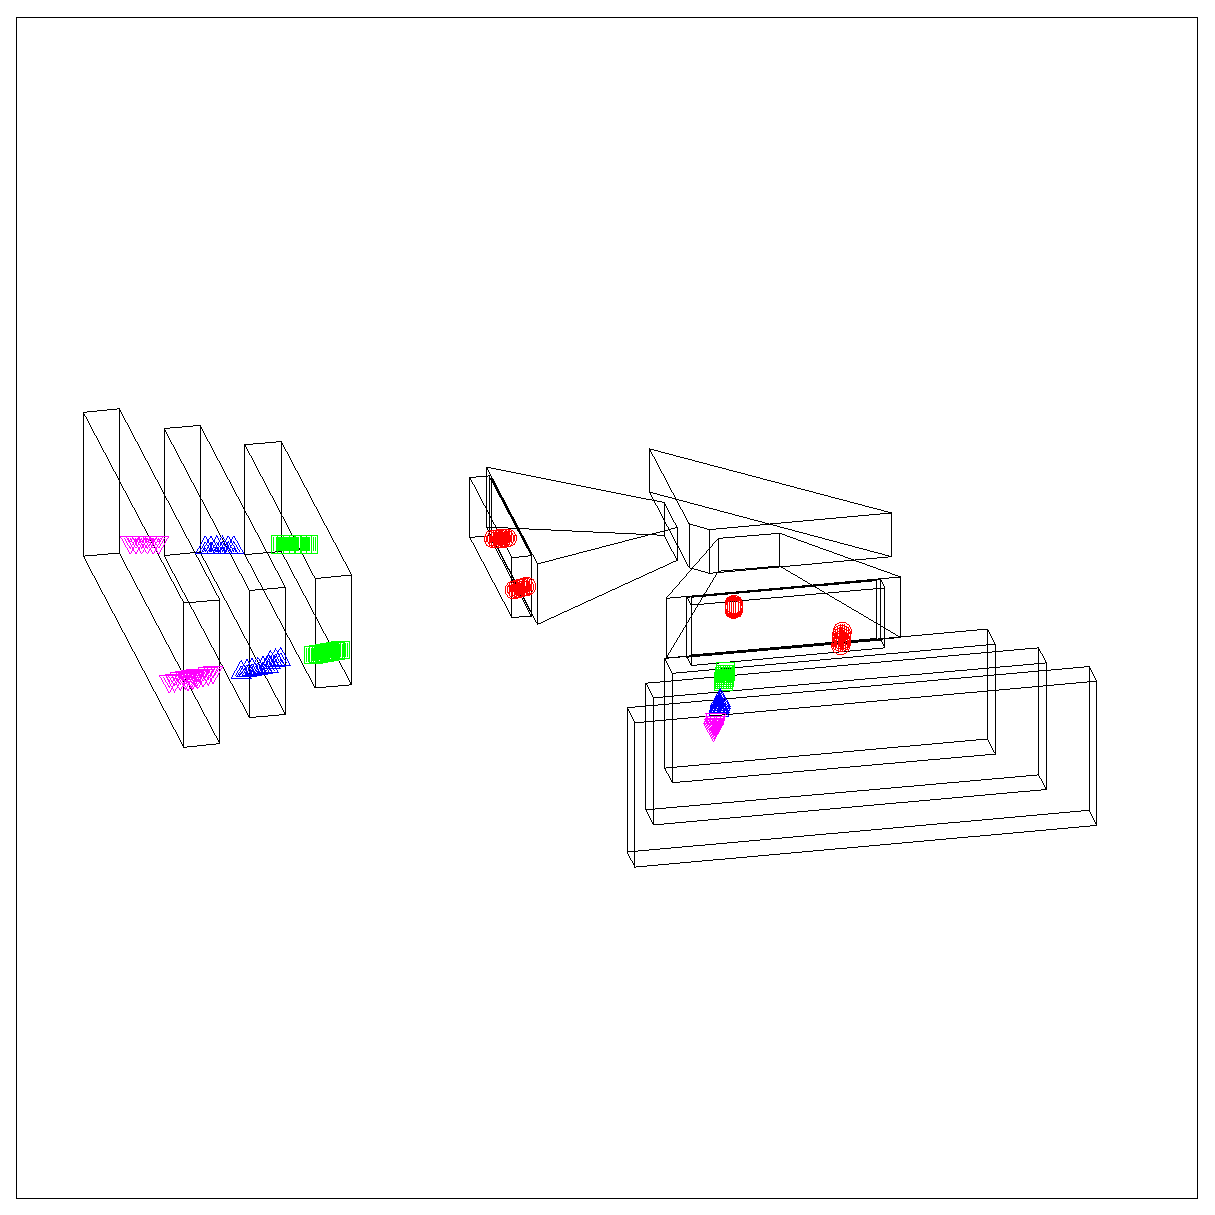
\epsfig{file=eps/draw140-1.eps,width=10cm}

\begin{verbatim}
 CALL GDRAW('CAVE',40.,40.,0.,10.,10.,.04,.04)
 CALL IGSET('TXCI',2.)
 CALL GDHITS('DRFT','FSP ',0,850,.3)
 CALL IGSET('TXCI',3.)
 CALL GDHITS('DRFT','RSP1',0,851,.3)
 CALL IGSET('TXCI',4.)
 CALL GDHITS('DRFT','RSP2',0,852,.3)
 CALL IGSET('TXCI',5.)
 CALL GDHITS('DRFT','RSP3',0,853,.3)
\end{verbatim}

     \caption{example of use of {\tt GDHITS}}
     \label{fg:draw140-1}
\end{figure}

{\bf Note:}
It is obligatory for the use of this routine that the spatial
{\tt MARS} (MAster Reference System) current coordinates of the hits are stored
as the first 3 elements of the hit {\tt [HITS200]}.
\begin{DLtt}{MMMMM}
\item[CHUSET] ({\tt CHARACTER*4}) user set identifier (if '*' all sets are taken)
\item[CHUDET] ({\tt CHARACTER*4}) user detector identifier (if '*' all 
detectors are taken)
\item[ITRA]   ({\tt INTEGER}) number of selected track (if 0 all tracks are taken)
\item[ISYMB]  ({\tt INTEGER}) character selection number (see table above)
\item[SSYMB]  ({\tt REAL}) size of characters in cm (if 0, a default of 
0.1 is taken)
\end{DLtt}
\Shubr{GDCHIT}{(CHUSET,CHUDET,ITRA,ISYMB,SIZMAX,IHIT,HITMIN,HITMAX)}
Draws the hit points as stored by \Rind{GSCHIT}, which were
generated by track {\tt ITRA} in detector {\tt CHUDET} of set {\tt CHUSET},
with the currently selected view parameters in \FCind{/GCDRAW/}.
Except for {\tt ISYMB = -1} the size of the character
is chosen as a function of {\tt HITS(IHIT)}:
\begin{center}
\ttfamily SIZE = sizmax * ( hits(ihit) - hitmin ) / hitmax
\end{center}

{\bf Note:}
It is obligatory for the use of this routine that the spatial
{\tt MARS} ({\tt MA}ster {\tt R}eference {\tt S}ystem) current coordinates 
of the hits are stored as the first 3 elements of the hit {\tt [HITS200]}.
\begin{DLtt}{MMMMM}
\item [SIZMAX]   ({\tt REAL}) maximum character size in cm
\item [IHIT]     ({\tt INTEGER}) {\tt HITS(IHIT)} contains the calorimeter 
hit value. {\tt IHIT>3}, and the first three elements are supposed to
contain the space position of the hit
\item [HITMIN]    ({\tt REAL}) minimum boundary of {\tt HITS(IHIT)}
\item[HITMAX]     ({\tt REAL}) maximum boundary of {\tt HITS(IHIT)}
\end{DLtt}
\Shubr{GDAHIT}{(X,Y,Z,ISYMB,SSYMB)}
Draws one hit point at coordinates {\tt X, Y, Z}. This routine is useful
when the user wants only to display but not to store the hits.
The first three arguments are the position of the hit in the {\tt MARS},
and the last two arguments have the same meaning as the similar 
arguments in GDHITS.
\begin{DLtt}{MM}
\item [X]  ({\tt REAL})       x coordinate in {\tt MARS} of the hit point
\item [Y]  ({\tt REAL})       y coordinate in {\tt MARS} of the hit point
\item [X]  ({\tt REAL})       z coordinate in {\tt MARS} of the hit point
\end{DLtt}

An example of use of the hits drawing routines is given in fig~\ref{fg:draw140-1}.
%\begin{verbatim}
%SUBROUTINE GUTREV
% - - - - -
% CALL GDOPT('THRZ','ON ')
% CALL GDRAWC('OPAL',2,5.,10.,10.,0.013,0.013)
% CALL GTREVE
% END
% 
% SUBROUTINE GUSTEP
% - - - - -
% CALL GDCXYZ
% - - - - -
% END
% 
% CALL GDOPT('THRZ','ON  ')
% CALL GDRAWC('OPAL',2,5.,10.,10.,0.013,0.013)
% CALL GDCHIT('EB  ',0,0,841,1.,6,0.,0.5)
% CALL GDCHIT('EE  ',0,0,841,1.,6,0.,0.5)
% CALL GDCHIT('HB  ',0,0,851,1.,5,0.,0.5)
% CALL GDCHIT('HE  ',0,0,851,1.,5,0.,0.5)
% CALL GDHITS('CJ  ',0,0,0,0.01)
% CALL GDHITS('CV  ',0,0,0,0.01)
% CALL GDHITS('CZ  ',0,0,0,0.01)
% CALL GDHITS('F   ',0,0,853,0.1)
% CALL GDHITS('HP  ',0,0,840,0.2)
% CALL GDHITS('ME  ',0,0,842,0.2)
% CALL GDHITS('MB  ',0,0,842,0.2)
%\end{verbatim}
% 
% 
